\documentclass[conference,onecolumn]{IEEEtran}
\usepackage[utf8]{inputenc}
\usepackage[T1]{fontenc}
\usepackage{cite}
\usepackage{amsmath,amssymb,amsfonts}
\usepackage{graphicx}
\usepackage{textcomp}
\usepackage{xcolor}
\usepackage{booktabs}
\usepackage{array}
\usepackage{tabularx}
\usepackage{tikz}
\usepackage{xurl}
\usepackage[colorlinks=true,linkcolor=black,citecolor=black,urlcolor=blue]{hyperref}
\urlstyle{same}

\urldef{\repourl}\nolinkurl{https://github.com/iimarky1234/LoRa-Weather-Station.git}
\urldef{\flowcharturl}\nolinkurl{https://github.com/iimarky1234/LoRa-Weather-Station/blob/baaa71d1f1d5a8bfd5d371a7b0f6451495bd53da/docs/FlowChart/System%20Architecture%20Flowcharts.pdf}
\urldef{\pwaurl}\nolinkurl{https://weather.iimarky123.io.vn/}

% Macros for AI Usage Declaration checkboxes (Page 9):
% Change \uncheckedbox to \checkedbox on any line you wish to tick.
\newcommand{\uncheckedbox}{$\square$}
\newcommand{\checkedbox}{\rlap{$\checkmark$}$\square$}

\newcolumntype{L}[1]{>{\raggedright\arraybackslash}p{#1}}
\newcolumntype{C}[1]{>{\centering\arraybackslash}p{#1}}
\newcolumntype{R}[1]{>{\raggedleft\arraybackslash}p{#1}}
\newcolumntype{Y}{>{\raggedright\arraybackslash}X}

\renewcommand{\topfraction}{0.92}
\renewcommand{\bottomfraction}{0.88}
\renewcommand{\textfraction}{0.06}
\renewcommand{\floatpagefraction}{0.85}
\setlength{\textfloatsep}{6pt plus 2pt minus 2pt}
\setlength{\floatsep}{5pt plus 2pt minus 2pt}
\setlength{\intextsep}{5pt plus 2pt minus 2pt}

\makeatletter
\newcommand{\linebreakand}{%
\end{@IEEEauthorhalign}%
\hfill\mbox{}\par
\mbox{}\hfill\begin{@IEEEauthorhalign}%
}
\makeatother

\begin{document}

\title{LoRa-Based Climate Monitoring System for Large-Scale Farms and Greenhouses}

\author{
\IEEEauthorblockN{Nguyen Luong Gia Triet}
\IEEEauthorblockA{\textit{FPT University - IA2014 - Group 2} \\
trietn31@gmail.com \\
ORCID: 0009-0006-2792-0802}
\and
\IEEEauthorblockN{Duong Duc Quang}
\IEEEauthorblockA{\textit{FPT University - IA2014 - Group 2} \\
duongquang2208@gmail.com \\
ORCID: 0009-0003-5452-9815}
\linebreakand
\IEEEauthorblockN{Phan Tan Anh Khoi}
\IEEEauthorblockA{\textit{FPT University - IA2014 - Group 2} \\
pkhoi6261@gmail.com \\
ORCID: 0009-0008-5517-5410}
\and
\IEEEauthorblockN{Nguyen Thai Thinh}
\IEEEauthorblockA{\textit{FPT University - IA2014 - Group 2} \\
nguyenthaithinh13092007@gmail.com \\
ORCID: 0009-0001-6356-5258}
}

\maketitle

\begin{abstract}
Large agricultural areas are usually located far from residential zones, where Wi-Fi coverage is unavailable and cellular networks (3G/4G) are unstable or expensive, while indoor greenhouse climate parameters (air temperature, humidity, and light intensity) change quickly and are difficult to track by hand. LoRa technology offers multi-kilometer wireless range, very low power use, and no regular mobile data fees for each node. This paper presents the design, implementation, and three-day field test of a low-power LoRa-based climate monitoring system for large-scale farms and greenhouses using the ESP32 (ESP32-S3-N16R8) microcontroller and the MKE-M24 Ra-02SH (Ai-Thinker Ra-02, Semtech SX1278) LoRa radio module. The sensor node connects five environmental sensors---AM2301B (air temperature and relative humidity), BH1750 (ambient light), LTR390 (UV index), Grove Soil Moisture Sensor, and APM10 (fine dust PM$_{1.0}$, PM$_{2.5}$, and PM$_{10}$)---along with an MKE-M09 RTC DS1307 for recording time and a 10,000 mAh Li-Po backup battery. A compact 26-byte binary protocol sends sensor data over LoRa (434.00 MHz, SF12, 15.6 kHz bandwidth, coding rate 4/5, and +20 dBm transmit power) to a central gateway with two permanent storage options (MicroSD card and 16 MB onboard flash backup), ThingSpeak cloud connection, and a local backup Progressive Web App (PWA) dashboard. Across a three-day test in a city environment (November 5--7, 2026), the system recorded 807 valid sensor data packets at a mean interval of 60.10 s with an average RSSI of $-76.77$ dBm and an average SNR of 9.05 dB, confirming stable data collection despite city buildings that limit current range to about 1 km.
\end{abstract}

\begin{IEEEkeywords}
Climate monitoring, ESP32-S3, greenhouse microclimate, Internet of Things (IoT), large-scale agriculture, LoRa, LoRaWAN, wireless sensor networks (WSN).
\end{IEEEkeywords}

\section{Introduction}
Environmental and weather monitoring supports agricultural planning, crop management, and natural disaster prevention \cite{dajnowski2024, hidayat2019, zennaro2025}, and keeping air temperature, relative humidity, and soil moisture in balance helps improve crop yield and quality \cite{dajnowski2024, hidayat2019, lopez2025}. However, collecting real-time climate data across many points remains difficult. Large-scale farms are spread across wide areas far from residential centers, where Wi-Fi is absent and cellular networks (3G/4G) often have weak coverage (``blank spots'') or require regular mobile data fees for every sensor node \cite{hidayat2019, zennaro2025, lopez2025, pietrosemoli2019}. Meanwhile, inside greenhouses, air temperature, relative humidity, and light intensity directly control plant growth and can change quickly; manual monitoring requires heavy labor, is not continuous, and is too slow to detect harmful conditions in time.

LoRa and LoRaWAN operate in free sub-GHz Industrial, Scientific, and Medical (ISM) frequency bands, send signals over several kilometers with very low power consumption \cite{dajnowski2024, murdyantoro2019}, and avoid per-node mobile data fees \cite{pietrosemoli2019}. This study is guided by the research question: \textit{How can a low-power climate monitoring system using LoRa technology be designed to stably collect environmental data in large-scale farms and greenhouses where Wi-Fi and cellular infrastructure is limited?} To answer this question, we review six published studies on LoRa/LoRaWAN weather monitoring \cite{dajnowski2024, hidayat2019, zennaro2025, lopez2025, pietrosemoli2019, murdyantoro2019}, build a complete ESP32-S3-N16R8 and LoRa monitoring system, and evaluate a three-day field dataset of 807 packets (November 5--7, 2026).

\smallskip
\noindent\textbf{Project Open-Source Repository, Live Web Dashboard, and System Flowcharts:}
\begin{itemize}
    \item \textbf{GitHub Repository (Source Code, Schematics \& Dataset):} \href{https://github.com/iimarky1234/LoRa-Weather-Station.git}{\textbf{\repourl}}
    \item \textbf{Live Monitoring Web Dashboard (PWA):} \href{https://weather.iimarky123.io.vn/}{\textbf{\pwaurl}}
    \item \textbf{System Architecture Flowcharts (GitHub PDF):}\\
    \href{https://github.com/iimarky1234/LoRa-Weather-Station/blob/baaa71d1f1d5a8bfd5d371a7b0f6451495bd53da/docs/FlowChart/System\%20Architecture\%20Flowcharts.pdf}{\resizebox{0.95\linewidth}{!}{\textbf{\flowcharturl}}}
\end{itemize}

\section{Literature Review}

\subsection{Comparison with Traditional Wireless Technologies}
Short-range wireless modules such as Bluetooth Low Energy (BLE), Zigbee, and Wi-Fi generally operate under 100 m \cite{murdyantoro2019}, and consumer weather stations such as the AcuRite 5-in-1 and La Crosse WS-2300 reach only 25--100 m to the indoor console \cite{pietrosemoli2019}. Extending Wi-Fi with special antennas is costly and needs constant power, which was unavailable in the high-Andean farming zones of \cite{lopez2025}. Also, cellular modems and satellite transmitters typically draw 4 W and 50 W versus about 0.1 mW for LoRaWAN \cite{zennaro2025}. Traditional weather stations can cost many thousands of dollars (a Kyrgyz news report cited USD 80,000) versus about USD 1,000 for IoT/LoRaWAN stations; cellular networks also add a regular cost per sensor, while LoRaWAN's recurring cost is limited to maintenance and the gateway's cellular service \cite{zennaro2025}. LoRa uses Chirp Spread Spectrum (CSS) modulation in sub-GHz ISM bands (433, 868, and 915 MHz) with strong resistance to interference \cite{lopez2025, murdyantoro2019}.

\subsection{LoRa Point-to-Point vs. LoRaWAN Star Network Structures}
Published LoRa weather monitoring systems use two main network structures:
\begin{itemize}
    \item \textbf{LoRaWAN star-of-stars:} Dajnowski et al. \cite{dajnowski2024}, Zennaro et al. \cite{zennaro2025}, and Pietrosemoli et al. \cite{pietrosemoli2019} send end-node packets to a multi-channel gateway (8-channel Dragino LPS8 \cite{dajnowski2024} or Milesight UG67 \cite{zennaro2025}), which forwards them over TCP/IP to Network and Application Servers \cite{dajnowski2024, zennaro2025, pietrosemoli2019}, such as The Things Network (TTN) \cite{dajnowski2024, pietrosemoli2019}. Dajnowski et al. describe AES128 encryption with three keys (\texttt{AppSKey}, \texttt{DevAddr}, \texttt{NwkSKey}) \cite{dajnowski2024}, while Pietrosemoli et al. note end-to-end encryption to the Application server \cite{pietrosemoli2019}.
    \item \textbf{Point-to-point (P2P) and gateway bridges:} Hidayat et al. \cite{hidayat2019}, Lopez et al. \cite{lopez2025}, and Murdyantoro et al. \cite{murdyantoro2019} connect transmitter nodes to a local receiver or gateway (a second ESP32 LoRa node \cite{hidayat2019, lopez2025} or an LG01-S gateway \cite{murdyantoro2019}) that uploads data over Wi-Fi \cite{hidayat2019, lopez2025, murdyantoro2019}. Hidayat et al. directly choose P2P LoRa \cite{hidayat2019}. Lopez et al. call their system LoRaWAN-based, but its architecture has only a sender node, a receiver node, and a custom IoT server without a LoRaWAN network server, so we group it with the P2P designs \cite{lopez2025}.
\end{itemize}

\subsection{Data Reliability, Visualization, and Transmission Range}
Because rural Internet is often unstable, Hidayat et al. \cite{hidayat2019} applied a Local/Global Management Subsystem (LMS/GMS) where the gateway uses an RTC DS3231 for timestamps and an SD card to save packets during outages before re-uploading. Similarly, Zennaro et al. \cite{zennaro2025} built a Disruption Tolerant Gateway (DTG) on a Milesight UG67 with MQTT QoS 2 (``exactly once'') whose internal memory holds over two years of messages from one station. For visualization, \cite{dajnowski2024} and \cite{murdyantoro2019} used ThingSpeak (up to 8 fields per channel, requiring multiple channels in \cite{dajnowski2024}), while \cite{zennaro2025} and \cite{lopez2025} use InfluxDB or Laravel REST API/MySQL with Grafana dashboards and email, Telegram, or WhatsApp alerts.

LoRa can reach 10 km or more in open areas \cite{dajnowski2024, murdyantoro2019}, depending on line of sight (LoS). In high-mountain Peru (3800--4000 m.a.s.l.), Lopez et al. \cite{lopez2025} achieved 100\% packet delivery over 10 km in LoS and 5 km in a rural area with scattered houses. In contrast, Hidayat et al. \cite{hidayat2019} tested 915 MHz TTGO LoRa32 modules among buildings and trees: LoS zone D reached 800 m (mean RSSI $-114$ dB, 20\% loss); tree/building zones A and C reached 400 m; and zone B behind a 39 m building reached only 200 m ($-124$ dB, 80\% loss).

\subsection{Embedded Hardware, Sensors, Power, and Literature Gaps}
Table~\ref{tab:comparison} compares the six reviewed systems with our design. Dajnowski et al. \cite{dajnowski2024} and Murdyantoro et al. \cite{murdyantoro2019} use Arduino boards, and \cite{dajnowski2024} noted that Arduino memory was stretched to its limits. Hidayat et al. \cite{hidayat2019}, Lopez et al. \cite{lopez2025}, and Pietrosemoli et al. (LoPy4) \cite{pietrosemoli2019} use ESP32 boards with sleep modes and built-in Wi-Fi \cite{hidayat2019, lopez2025}. For temperature, humidity, and pressure, \cite{dajnowski2024, hidayat2019, pietrosemoli2019, murdyantoro2019} use DHT11, DHT22, BMP180, and BME280 sensors, \cite{lopez2025} uses industrial RS485 sensors, and \cite{zennaro2025} uses the WMO-standard MeteoHelix IoT PRO. Light is measured by TSL2561 \cite{hidayat2019}, a solar radiation sensor \cite{lopez2025}, or a small solar panel \cite{zennaro2025}, with no dedicated UV index sensor in any study. Soil sensing appears only in \cite{zennaro2025} (SenseCAP S2105) and \cite{lopez2025} (DS18B20 soil temperature, with soil moisture listed as a target variable). For air quality, \cite{dajnowski2024} uses an MQ-135 gas sensor ($\text{CO}_2$, CO, $\text{NH}_3$, $\text{NO}_x$, smoke), and \cite{zennaro2025} mentions $\text{PM}_{2.5}/\text{PM}_{10}$ only in an undeployed 10-in-1 sensor (SenseCAP S1000 V2). Five studies measure wind or rain \cite{dajnowski2024, zennaro2025, lopez2025, pietrosemoli2019, murdyantoro2019}. For low power, \cite{pietrosemoli2019} turns off the 433 MHz receiver (9.9 mA) before deep sleep (32.8 $\mu$A), and \cite{lopez2025} uses a relay to cut sensor power during sleep (95--120 s) with a 10--15 s warm-up. This review reveals three gaps: (1) no study tests in a greenhouse or combines air temperature/humidity, light, UV index, soil moisture, and fine dust ($\text{PM}_{1.0}$, $\text{PM}_{2.5}$, $\text{PM}_{10}$) in one low-cost node; (2) Arduino stations face memory limits \cite{dajnowski2024} or lack local backup storage \cite{murdyantoro2019}; and (3) direct-powered stations still need battery backup and sleep management during power cuts \cite{zennaro2025}.

\begin{table}[!htbp]
\centering
\caption{Comparison of Reviewed LoRa/LoRaWAN Weather Monitoring Systems and Proposed Project Design}
\label{tab:comparison}
\scriptsize
\setlength{\tabcolsep}{3.5pt}
\renewcommand{\arraystretch}{0.91}
\begin{tabularx}{\textwidth}{L{1.8cm} L{2.4cm} L{3.8cm} L{2.8cm} L{2.5cm} Y}
\toprule
\textbf{Study} & \textbf{MCU \& LoRa} & \textbf{Parameters \& Sensors} & \textbf{Network \& Storage} & \textbf{Power} & \textbf{Range \& Findings / Limitations} \\
\midrule
Dajnowski et al. (2024) \cite{dajnowski2024} & Arduino MCU, Dragino LoRa shield, LPS8 gateway & Temp., humidity (DHT-11/22; BME280 alt.), pressure, wind, rain, light, air quality (MQ-135) & LoRaWAN, TTN, ThingSpeak, Flask web GUI & Battery (solar proposed as future work) & No range test (1--10 km quoted); Arduino memory limits; condensation; fast battery drain. \\
Hidayat et al. (2019) \cite{hidayat2019} & ESP32 TTGO LoRa32 V2 (sender \& gateway) & Temp., humidity (DHT22), light (TSL2561) & P2P LoRa 915 MHz to Wi-Fi gateway; RTC DS3231 + SD card & Battery + deep sleep & 800 m in LoS (20\% loss); 200--400 m with buildings/trees (up to 80\% loss). \\
Zennaro et al. (2025) \cite{zennaro2025} & Commercial LoRaWAN nodes, Milesight UG67 DTG & Temp., humidity, pressure, irradiation (MeteoHelix), wind, rain, soil moisture (S2105), tilt, river level & LoRaWAN to cellular via MQTT QoS 2; InfluxDB, Grafana & MeteoHelix: solar + Li-ion; gateway: 305 Wp solar + 100 Ah battery & Links to 1.5 km (Tatyr); temp. within 0.5$^\circ$C of reference 96.2\% of the time. \\
Lopez et al. (2025) \cite{lopez2025} & ESP32 WROOM 32, Ebyte E220-900T22D, MAX485 & Air temp./humidity (CWT-TH04S), soil temp. (DS18B20), solar rad., wind; soil moisture, pressure listed & LoRa 915 MHz to ESP32 Wi-Fi receiver; Laravel REST API, MySQL, Grafana & 37 W solar panel, 8000 mAh 18650 battery, sleep + sensor relay & 10 km (LoS), 5 km (scattered houses), 100\% delivery; cost $\sim$USD 320. \\
Pietrosemoli et al. (2019) \cite{pietrosemoli2019} & BSF32 or LoPy4 (ESP32), SX1276, RXB6 433 MHz receiver & Intercepts AcuRite/La Crosse sensors (temp., humidity, wind, rain) + BMP180 pressure & 433 MHz bridged to 868 MHz LoRaWAN (TTN) & BSF32: 2000 mAh Li-ion; LoPy4: 48 Wh pack, 32.8 $\mu$A sleep & No field range test; est. battery life 123 days (BSF32), 414 days (LoPy4) at 15 min. \\
Murdyantoro et al. (2019) \cite{murdyantoro2019} & Arduino UNO Rev3, LoRa shield, LG01-S gateway & Temp., humidity (DHT11), pressure (BMP180), raindrop sensor, 3-cup anemometer & LoRa 915 MHz (SF9) to Wi-Fi gateway; ThingSpeak & Power bank & Two nodes matched ThingSpeak; 5--10 km quoted, not measured; no local backup, soil, UV, or dust. \\
\textbf{Proposed (Group 2)} & ESP32 (ESP32-S3-N16R8), MKE-M24 Ra-02SH (SX1278), 525 MHz 3.5 dBi antenna & Air temp./humidity (AM2301B), light (BH1750), UV (LTR390), soil moisture (Grove), fine dust PM$_{1.0}$/PM$_{2.5}$/PM$_{10}$ (APM10) & LoRa P2P (434 MHz, SF12); RTC DS1307, MicroSD + 16 MB Flash backup, ThingSpeak \& Local PWA & Direct power + 10,000 mAh Li-Po backup + deep sleep & Theoretical 5--10 km (rural), $\sim$1 km (urban tests, 807 packets, mean RSSI $-76.77$ dBm); no wind sensor. \\
\bottomrule
\end{tabularx}
\end{table}

\section{System Architecture and Hardware Design}

\subsection{Overall System Architecture}
Figure~\ref{fig:block_diagram} shows the system block diagram, which separates field sensing from Internet upload using a \textbf{Weather Station Node} in the farm or greenhouse and a \textbf{Central Gateway} where Wi-Fi access is available. In addition to the Node and Gateway (\texttt{firmware/node/} and \texttt{firmware/gateway/}), our repository also provides an all-in-one \textbf{Standalone Station} (\texttt{firmware/standalone/}) for single-board local logging and cloud upload without LoRa, as well as a \textbf{Repeater} workflow in the system design flowcharts to forward packets across longer distances.

\begin{figure}[!htbp]
\centering
\IfFileExists{Official_Block_Diagram.png}{%
    \includegraphics[trim=0 0 0 518,clip,width=0.88\textwidth]{Official_Block_Diagram.png}%
}{%
    \fbox{\parbox[c][0.19\textheight][c]{0.88\textwidth}{\centering \textbf{Official\_Block\_Diagram.png}\\(Upload \texttt{Official\_Block\_Diagram.png} to Overleaf project root)}}%
}
\caption{System block diagram of the ESP32-based Weather Station Node and Central Gateway showing $\text{I}^2\text{C}$ addresses (\texttt{0x23}, \texttt{0x68}, \texttt{0x38}, \texttt{0x1C}), ADC, UART, SPI1/SPI2 buses, status LED colors, and Cloud/Localhost paths.}
\label{fig:block_diagram}
\end{figure}

As shown in Fig.~\ref{fig:block_diagram}, the Weather Station Node uses an ESP32 (\textbf{ESP32-S3-N16R8}) to read three sensor interfaces: a shared $\text{I}^2\text{C}$ bus for Ambient Light (\texttt{0x23}), Real-Time Clock (\texttt{0x68}), Temperature/Humidity (\texttt{0x38}), and UV (\texttt{0x1C}); an analog ADC channel for Soil Moisture; and a UART interface for the Particulate Matter sensor. Readings are packed into a 26-byte binary packet and sent via LoRa on \texttt{SPI1}. The Central Gateway receives LoRa packets via \texttt{SPI1}, saves CSV records to a MicroSD card on \texttt{SPI2} (with automatic 16 MB internal flash backup), displays system status on its built-in RGB LED (Green for Cloud, Blue for Received LoRa, Yellow for Localhost Dashboard, Red for Error), and forwards data over Wi-Fi to ThingSpeak Cloud or a local web dashboard.

\subsection{Sensor Node and Central Gateway Circuit Schematics}
Figures~\ref{fig:schematic_node} and \ref{fig:schematic_gateway} show the Sensor Node and Central Gateway circuit schematics (\textit{Rev. 1.0}), and Table~\ref{tab:pinout} summarizes the hardware connections and LoRa radio settings. Each station is built from the project hardware list: one unit each (\texttt{1c}) of ESP32 (\texttt{ESP32-S3-N16R8}), \textbf{AM2301B} temperature and humidity sensor (\texttt{H3 AM2301b}), \textbf{MKE-M24 Ra-02SH} LoRa module (\texttt{L1 RA-02SH}, Ai-Thinker Ra-02 / Semtech SX1278), \textbf{BH1750} $\text{I}^2\text{C}$ light sensor (\texttt{1 LIGHT-SENSOR-BH1750}), \textbf{Grove Soil Moisture Sensor} (\texttt{4 SOIL-MOISTURE-SENSOR}), \textbf{525 MHz 3.5 dBi} LoRa antenna, \textbf{MKE-M09 RTC DS1307} (\texttt{U2 DS1307\_RTC}), \textbf{MicroSD reader} (\texttt{U3 MICROSD\_READER}), \textbf{LTR390} UV sensor (\texttt{H2 LTR390 UV Light}), \textbf{APM10} fine dust sensor (\texttt{H1 APM10}), and a \textbf{10,000 mAh Li-Po battery}.

\begin{figure}[!htbp]
\centering
\IfFileExists{Schematic Node.png}{%
    \includegraphics[trim=169 177 99 182,clip,width=0.78\textwidth]{Schematic Node.png}%
}{%
    \fbox{\parbox[c][0.22\textheight][c]{0.78\textwidth}{\centering \textbf{Schematic Node.png}\\(Upload \texttt{Schematic Node.png} to Overleaf project root)}}%
}
\caption{Circuit schematic of the Sensor Node (\texttt{U4 ESP32-S3-N16R8}, \texttt{L1 RA-02SH}, \texttt{U2 DS1307\_RTC}, \texttt{1 LIGHT-SENSOR-BH1750}, \texttt{3 LOGIC-LEVEL-CONVERTER}, \texttt{4 SOIL-MOISTURE-SENSOR}, \texttt{H1 APM10}, \texttt{H2 LTR390 UV Light}, and \texttt{H3 AM2301b}).}
\label{fig:schematic_node}
\end{figure}

\begin{figure}[!htbp]
\centering
\IfFileExists{Schematic Gateway.png}{%
    \includegraphics[trim=374 231 320 162,clip,width=0.42\textwidth]{Schematic Gateway.png}%
}{%
    \fbox{\parbox[c][0.21\textheight][c]{0.42\textwidth}{\centering \textbf{Schematic Gateway.png}\\(Upload \texttt{Schematic Gateway.png} to Overleaf project root)}}%
}
\caption{Circuit schematic of the Central Gateway (\texttt{U4 ESP32-S3-N16R8}, \texttt{L1 RA-02SH} on \texttt{SPI1}, and \texttt{U3 MICROSD\_READER} on separate \texttt{SPI2}).}
\label{fig:schematic_gateway}
\end{figure}

On the Sensor Node (Fig.~\ref{fig:schematic_node}), the shared 100 kHz $\text{I}^2\text{C}$ bus on \texttt{GPIO8} (\texttt{SDA}) and \texttt{GPIO9} (\texttt{SCL}) connects the \texttt{DS1307} RTC, \texttt{BH1750}, \texttt{LTR390}, and \texttt{AM2301B} sensors powered from the \texttt{3V3} pin. The Grove Soil Moisture analog output (\texttt{AO}) connects to \texttt{GPIO6} (0--3.3 V ADC input, calibrated in \texttt{drivers/soil.py} between 2800 mV dry and 1200 mV wet). Because the \texttt{APM10} dust sensor uses 5.0 V power while the ESP32-S3 uses 3.3 V logic, a \textbf{Logic-Level Converter} (\texttt{3 LOGIC-LEVEL-CONVERTER}) safely shifts the 1200-baud UART lines between \texttt{GPIO10} (\texttt{TX}) and \texttt{GPIO14} (\texttt{RX}) on the ESP32-S3 and the \texttt{APM10} sensor. The station runs on direct electrical power with the 10,000 mAh Li-Po battery as backup during power cuts.

On both the Node and Gateway, the \texttt{RA-02SH} LoRa module connects to the ESP32-S3 via \texttt{SPI1}: \texttt{SCK} to \texttt{GPIO18}, \texttt{MISO} to \texttt{GPIO13}, \texttt{MOSI} to \texttt{GPIO11}, \texttt{NSS} (\texttt{CS}) to \texttt{GPIO2}, and \texttt{RESET} to \texttt{GPIO3} (with the interrupt line wired to \texttt{GPIO5} on the Node schematic and \texttt{GPIO6} on the Gateway). On the Central Gateway (Fig.~\ref{fig:schematic_gateway}), the \texttt{MICROSD\_READER} uses a separate \texttt{SPI2} bus on \texttt{GPIO36} (\texttt{SCK}), \texttt{GPIO35} (\texttt{MOSI}), \texttt{GPIO37} (\texttt{MISO}), and \texttt{GPIO4} (\texttt{CS}) so that reading or writing CSV files on the MicroSD card never interferes with incoming LoRa packets on \texttt{SPI1}.

\begin{table}[!htbp]
\centering
\caption{ESP32-S3-N16R8 Hardware Pinout Mapping and SX1278 LoRa Radio Settings}
\label{tab:pinout}
\scriptsize
\setlength{\tabcolsep}{4pt}
\renewcommand{\arraystretch}{0.91}
\begin{tabularx}{\textwidth}{L{3.0cm} L{2.4cm} L{3.9cm} Y}
\toprule
\textbf{Subsystem / Parameter} & \textbf{ESP32-S3 Pin / Value} & \textbf{Connected Component} & \textbf{Interface \& Function in System} \\
\midrule
\multicolumn{4}{l}{\textit{\textbf{Part A: Sensor Node \& Central Gateway Hardware Pinout (ESP32-S3-N16R8)}}} \\
Shared $\text{I}^2\text{C}$ Bus (Node) & \texttt{GPIO8 (SDA), GPIO9 (SCL)} & DS1307, BH1750, LTR390, AM2301B & 100 kHz $\text{I}^2\text{C}$ bus (addresses \texttt{0x68}, \texttt{0x23}, \texttt{0x1C}, \texttt{0x38}) \\
APM10 UART (Node) & \texttt{GPIO10 (TX), GPIO14 (RX)} & APM10 Dust Sensor (via Level Shifter) & 1200-baud UART reading PM$_{1.0}$, PM$_{2.5}$, and PM$_{10}$ (3.3 V $\leftrightarrow$ 5 V) \\
Soil Moisture ADC (Node) & \texttt{GPIO6} & Grove Soil Moisture Sensor (\texttt{AO}) & Analog ADC input (0--3.3 V; 2800 mV dry to 1200 mV wet) \\
LoRa SPI1 Bus (Both) & \texttt{GPIO18 / 11 / 13} & Ra-02SH \texttt{SCK / MOSI / MISO} & Dedicated \texttt{SPI1} bus for LoRa radio communication \\
LoRa Control Pins (Both) & \texttt{GPIO2 (CS), GPIO3 (RST)} & Ra-02SH \texttt{NSS / RESET} (\& \texttt{DIO}) & Chip Select and Reset (\texttt{GPIO5} on Node; \texttt{GPIO6} on Gateway) \\
MicroSD SPI2 (Gateway) & \texttt{GPIO36 / 35 / 37 / 4} & MicroSD \texttt{SCK / MOSI / MISO / CS} & Separate \texttt{SPI2} bus for CSV data logging to MicroSD card \\
Status RGB LED (Both) & \texttt{GPIO48 / GPIO38} & Built-in WS2812 RGB LED & Displays Green, Yellow, Blinking Grey, Blue Flash, or Red \\
Power Pins (Both) & \texttt{3V3, 5V, GND} & Sensors, RTC, Level Shifter, Ra-02SH, SD & 3.3 V for MCU/sensors/LoRa; 5.0 V for APM10 and Level Shifter \\
\midrule
\multicolumn{4}{l}{\textit{\textbf{Part B: LoRa Radio Configuration (\texttt{firmware/node/config.py} \& \texttt{firmware/gateway/config.py})}}} \\
Carrier Frequency & \texttt{434.00 MHz} & MKE-M24 Ra-02SH (SX1278) & License-free sub-GHz ISM frequency band \\
Spreading Factor \& BW & \texttt{SF12}, \texttt{15.6 kHz} & MKE-M24 Ra-02SH (SX1278) & High spreading factor and narrow bandwidth for long range \\
Coding Rate \& Preamble & \texttt{4/5}, \texttt{8 symbols} & MKE-M24 Ra-02SH (SX1278) & Forward error correction and packet synchronization header \\
Transmit Power \& Sync & \texttt{+20 dBm}, \texttt{0x12} & MKE-M24 Ra-02SH (SX1278) & Maximum 100 mW transmit power and private network sync word \\
Low Data Rate Opt. & \texttt{Enabled (Auto)} & MKE-M24 Ra-02SH (SX1278) & Keeps clock synchronization stable during slow \texttt{SF12} packets \\
\bottomrule
\end{tabularx}
\end{table}

\section{Firmware Architecture and Communication Protocol}

\subsection{LoRa Radio Configuration and 26-Byte Binary Protocol}
As shown in Table~\ref{tab:pinout} (Part B), both the Sensor Node and Central Gateway configure their SX1278 LoRa modules (\texttt{common/sx1278.py}) with the same radio parameters in \texttt{config.py}: \texttt{434.00 MHz} frequency, spreading factor \texttt{SF12}, \texttt{15.6 kHz} bandwidth, coding rate \texttt{4/5}, and \texttt{+20 dBm} transmit power. Choosing \texttt{SF12} and +20 dBm gives the radio signal strong penetration through greenhouse frames, trees, and buildings. Because \texttt{SF12} sends data slowly to achieve long range, sending long JSON text strings would take too much airtime and battery power. Instead, \texttt{common/protocol.py} packs all sensor readings into a compact \textbf{26-byte binary packet}. Table~\ref{tab:protocol} shows the exact byte layout and ThingSpeak cloud field mapping. To keep two decimal places without using large floating-point numbers, decimal readings (temperature, relative humidity, soil moisture, and UV index) are multiplied by 100 before packing and divided by 100 when decoded at the Gateway.

\begin{table}[!htbp]
\centering
\caption{26-Byte Binary LoRa Packet Structure (\texttt{common/protocol.py}) and ThingSpeak Cloud Field Mapping}
\label{tab:protocol}
\scriptsize
\setlength{\tabcolsep}{4pt}
\renewcommand{\arraystretch}{0.91}
\begin{tabularx}{\textwidth}{C{1.6cm} L{2.8cm} C{1.1cm} L{3.3cm} L{3.5cm} Y}
\toprule
\textbf{Byte Offset} & \textbf{Field Name} & \textbf{Size} & \textbf{Binary Encoding} & \textbf{Measurement Unit / Resolution} & \textbf{ThingSpeak Cloud Field Mapping} \\
\midrule
\texttt{0} & Node ID & 1 Byte & Whole number (1--255) & Station identifier (\texttt{node\_id = 1}) & Selects Node 1 or Node 2 channel \\
\texttt{1 -- 2} & Sequence Number & 2 Bytes & Whole number (0--65,535) & Packet counter (\texttt{seq}) & Saved in ESP32 RTC memory \\
\texttt{3} & Mesh Hops & 1 Byte & Whole number (0--255) & Repeater hop count (\texttt{hops}) & Tracks repeater forwarding steps \\
\texttt{4 -- 7} & Timestamp & 4 Bytes & Unix epoch seconds & Seconds since 1970-01-01 (1 s step) & Converted to \texttt{YYYY-MM-DD HH:MM:SS} \\
\texttt{8 -- 9} & Air Temperature & 2 Bytes & $\text{Temperature} \times 100$ (signed) & Degrees Celsius ($0.01\,^\circ\text{C}$ step) & \textbf{Field 1:} Temperature ($^\circ$C) \\
\texttt{10 -- 11} & Relative Humidity & 2 Bytes & $\text{Humidity} \times 100$ & Percent $0.00\text{--}100.00\%$ ($0.01\%$ step) & \textbf{Field 2:} Relative Humidity (\%) \\
\texttt{12 -- 13} & Ambient Light & 2 Bytes & Whole number Lux & Illuminance in Lux ($1\text{ Lux}$ step) & \textbf{Field 3:} Ambient Light (Lux) \\
\texttt{14 -- 15} & Soil Moisture & 2 Bytes & $\text{Soil Moisture} \times 100$ & Percent $0.00\text{--}100.00\%$ ($0.01\%$ step) & \textbf{Field 8:} Soil Moisture (\%) \\
\texttt{16 -- 17} & UV Raw Count & 2 Bytes & Whole number sensor count & Raw LTR390 UV count & Internal UV sensor check \\
\texttt{18 -- 19} & UV Index & 2 Bytes & $\text{UV Index} \times 100$ & UV Index ($0.01\text{ UVI}$ step) & \textbf{Field 4:} Ultraviolet Index (UVI) \\
\texttt{20 -- 21} & Fine Dust PM$_{1.0}$ & 2 Bytes & Whole number concentration & $\mu\text{g/m}^3$ ($1\,\mu\text{g/m}^3$ step) & \textbf{Field 7:} PM$_{1.0}$ ($\mu\text{g/m}^3$) \\
\texttt{22 -- 23} & Fine Dust PM$_{2.5}$ & 2 Bytes & Whole number concentration & $\mu\text{g/m}^3$ ($1\,\mu\text{g/m}^3$ step) & \textbf{Field 5:} PM$_{2.5}$ ($\mu\text{g/m}^3$) \\
\texttt{24 -- 25} & Fine Dust PM$_{10}$ & 2 Bytes & Whole number concentration & $\mu\text{g/m}^3$ ($1\,\mu\text{g/m}^3$ step) & \textbf{Field 6:} PM$_{10}$ ($\mu\text{g/m}^3$) \\
\bottomrule
\end{tabularx}
\end{table}

\subsection{Firmware Workflows, Power Saving, and Web Dashboard}
For easy viewing, the four official system architecture flowcharts (\textit{Flowchart 1 --- Standalone Sensor}, \textit{Flowchart 2 --- Gateway}, \textit{Flowchart 3 --- Repeater}, and \textit{Flowchart 4 --- Sensor Node}) are linked on a separate line below:

\smallskip
\noindent\href{https://github.com/iimarky1234/LoRa-Weather-Station/blob/baaa71d1f1d5a8bfd5d371a7b0f6451495bd53da/docs/FlowChart/System\%20Architecture\%20Flowcharts.pdf}{\textbf{System Architecture Flowcharts (Click to Open GitHub PDF):}}\\
\noindent\href{https://github.com/iimarky1234/LoRa-Weather-Station/blob/baaa71d1f1d5a8bfd5d371a7b0f6451495bd53da/docs/FlowChart/System\%20Architecture\%20Flowcharts.pdf}{\resizebox{0.96\linewidth}{!}{\textbf{\flowcharturl}}}
\smallskip

\begin{enumerate}
    \item \textbf{Sensor Node (\texttt{firmware/node/}, Flowchart 4):} On startup or wake-up from deep sleep, \texttt{node/main.py} loads \texttt{node/config.py}, reads the saved packet sequence counter from the ESP32 RTC memory, turns on the status LED, and initializes the $\text{I}^2\text{C}$ bus, the six sensor drivers (\texttt{ds1307.py}, \texttt{bh1750.py}, \texttt{am2301b.py}, \texttt{ltr390.py}, \texttt{apm10.py}, and \texttt{soil.py}), and the SX1278 LoRa module. In each cycle, it reads the timestamp from the DS1307 RTC (or uses the system clock if the RTC is offline) and collects measurements from all five environmental sensors (using safe zero defaults if any sensor fails to respond). It then packs the data into a 26-byte binary frame (\texttt{common/protocol.py}), flashes the Blue LED, and sends the packet over LoRa (\texttt{lora.send()}). Although the system flowchart also outlines an optional ACK and retry loop, the deployed firmware uses a direct broadcast mode to minimize radio on-time: once transmission finishes, it increments and saves the sequence counter to RTC memory, puts the LoRa chip into sleep mode (\texttt{lora.sleep()}, $\sim 0.2\,\mu\text{A}$), turns off the RGB LED, and enters ESP32 deep sleep (\texttt{machine.deepsleep()}) for \texttt{TX\_INTERVAL\_SEC = 60} seconds.
    \item \textbf{Central Gateway (\texttt{firmware/gateway/}, Flowchart 2):} At boot, \texttt{gateway/main.py} loads \texttt{gateway/config.py}, initializes the status LED, and sets up dual storage (\texttt{gateway/storage.py}). It first tries to mount the MicroSD card (\texttt{/sd/gateway\_weather\_log.csv}); if no card is inserted or a write error happens later, it automatically switches to the 16 MB internal flash memory (\texttt{/gateway\_weather\_log.csv}) while also keeping the 50 newest records in a RAM buffer. Next, it initializes the SX1278 receiver and tries to connect to Wi-Fi for up to 12 seconds (blinking the Grey LED). Two asynchronous tasks then run in parallel:
    \begin{itemize}
        \item \textit{LoRa Receiver Task:} Keeps the SX1278 in continuous receive mode. Whenever a valid 26-byte packet arrives with a valid hardware CRC check, it reads the packet's \texttt{RSSI} and \texttt{SNR}, flashes the Blue LED, appends a CSV row to the MicroSD card (or internal flash), and updates the latest node data in memory.
        \item \textit{Cloud and Failover Web Task:} When Wi-Fi is connected (\textbf{Online Mode}, Solid Green LED), the gateway uploads new sensor data to ThingSpeak every 20 seconds (Channel \texttt{3543024} for Node 1 and Channel \texttt{3558474} for Node 2) while keeping the local web server off to save memory. If Wi-Fi fails at boot, the gateway starts a local Wi-Fi hotspot (\texttt{WeatherStation-ESP32} at \texttt{192.168.4.1}) with a captive portal DNS server (\texttt{dns\_server.py}) and local web dashboard (\texttt{web\_server.py}, Solid Yellow LED). Similarly, if ThingSpeak fails 3 times in a row during normal operation, the gateway automatically opens the local web dashboard at \texttt{http://<local\_ip>/} (Solid Yellow LED) and retries ThingSpeak every 60 seconds, switching back to Online Mode (Solid Green LED) once the cloud connection recovers.
    \end{itemize}
    \item \textbf{Standalone Station (\texttt{firmware/standalone/}, Flowchart 1):} Designed for single-location setups where LoRa is not needed, \texttt{standalone/main.py} connects the sensors and MicroSD card directly to one ESP32-S3 board. It syncs the DS1307 RTC with an Internet NTP time server (\texttt{pool.ntp.org}, UTC+7) at boot, reads all sensors every 20 seconds, saves CSV logs to MicroSD or internal flash, uploads to ThingSpeak, and uses the same automatic Yellow-LED local web dashboard fallback if Wi-Fi or ThingSpeak goes offline.
    \item \textbf{Repeater (Flowchart 3):} To extend range past obstacles, the system architecture includes a Repeater workflow supported by the \texttt{hops} field (Byte 3) in \texttt{common/protocol.py}. A repeater listens in continuous receive mode, checks packet validity, drops duplicate packets or packets that have reached the maximum hop limit, increases the hop count by one, waits a short random delay to avoid signal collisions, and re-transmits the packet toward the Central Gateway.
\end{enumerate}

In addition to the built-in local dashboard on the ESP32-S3 (\texttt{web\_server.py}, which serves \texttt{/}, \texttt{/api/data}, \texttt{/api/history}, and \texttt{/download}), the project provides a public cloud-synced Progressive Web App (\texttt{webapp/index.html}, live at \href{https://weather.iimarky123.io.vn/}{\textbf{\pwaurl}}). It displays an interactive map of sensor nodes, live sensor cards, historical charts, active storage status (\texttt{MicroSD (/sd)}, \texttt{Internal Flash (16MB)}, or \texttt{RAM Buffer Only}), and one-click CSV data downloads.

\section{Experimental Setup and Field Results}

\subsection{Three-Day City Test and Dataset Collection}
The prototype (Node 1, \texttt{node\_id = 1}, sending data to the Central Gateway) was tested in an urban environment over three consecutive days (November 5--7, 2026). All received packets were saved in \texttt{gateway\_weather\_log.csv}, producing \textbf{807 valid sensor data records} with zero missing or corrupted values:
\begin{itemize}
    \item \textbf{Day 1 (2026-11-05):} $n = 261$ records from \texttt{12:29:13} to \texttt{16:48:15} (4 h 19 min 02 s); time between packets ranged from 48.0 s to 72.0 s with a mean of 59.78 s ($\text{SD} = 7.38\text{ s}$).
    \item \textbf{Day 2 (2026-11-06):} $n = 273$ records from \texttt{12:26:06} to \texttt{16:58:55} (4 h 32 min 49 s); time between packets ranged from 48.0 s to 72.0 s with a mean of 60.18 s ($\text{SD} = 7.27\text{ s}$).
    \item \textbf{Day 3 (2026-11-07):} $n = 273$ records from \texttt{12:05:25} to \texttt{16:38:52} (4 h 33 min 27 s); time between packets ranged from 48.0 s to 72.0 s with a mean of 60.32 s ($\text{SD} = 7.10\text{ s}$).
\end{itemize}
Across all 804 within-day intervals, the overall mean interval was \textbf{60.10 s} ($\text{SD} = 7.24\text{ s}$), matching the 60-second deep-sleep cycle configured in \texttt{node/config.py}. Table~\ref{tab:dataset} summarizes the overall and daily statistics, and Fig.~\ref{fig:dataset_chart} plots the 30-minute average line charts (\texttt{12:00} to \texttt{16:30}) across all $N = 807$ records.

\begin{table}[!htbp]
\centering
\caption{Statistical Summary of the Three-Day Field Test Dataset (\texttt{gateway\_weather\_log.csv}, Node 1, $N = 807$ Records; Daily Columns Report $\text{Mean} \pm \text{SD}$)}
\label{tab:dataset}
\scriptsize
\setlength{\tabcolsep}{3.5pt}
\renewcommand{\arraystretch}{0.92}
\begin{tabularx}{\textwidth}{L{2.55cm} R{0.85cm} R{1.05cm} R{1.05cm} R{1.00cm} R{0.95cm} R{2.25cm} R{2.25cm} Y}
\toprule
\textbf{Parameter (Unit)} & \textbf{Min} & \textbf{Max} & \textbf{Mean} & \textbf{Median} & \textbf{SD} & \textbf{Day 1 ($n=261$)} & \textbf{Day 2 ($n=273$)} & \textbf{Day 3 ($n=273$)} \\
\midrule
Temperature ($^\circ$C) & 28.50 & 34.24 & 31.98 & 32.16 & 1.32 & $32.00 \pm 1.36$ & $32.03 \pm 1.29$ & $31.92 \pm 1.30$ \\
Relative Humidity (\%) & 59.92 & 95.66 & 70.23 & 67.66 & 8.42 & $70.17 \pm 8.56$ & $69.86 \pm 8.45$ & $70.67 \pm 8.25$ \\
Ambient Light (Lux) & 2047.90 & 64645.80 & 33549.71 & 32016.90 & 21083.72 & $32532.12 \pm 20992.79$ & $32288.32 \pm 20635.35$ & $35783.96 \pm 21507.07$ \\
Soil Moisture (\%) & 47.20 & 92.80 & 64.68 & 53.00 & 18.57 & $65.19 \pm 18.72$ & $66.08 \pm 19.00$ & $62.80 \pm 17.91$ \\
UV Index (UVI) & 0.00 & 8.46 & 4.25 & 4.10 & 2.67 & $4.11 \pm 2.67$ & $4.09 \pm 2.61$ & $4.54 \pm 2.71$ \\
PM$_{1.0}$ ($\mu\text{g/m}^3$) & 3.00 & 21.00 & 12.73 & 13.00 & 3.61 & $12.59 \pm 3.68$ & $12.80 \pm 3.63$ & $12.78 \pm 3.52$ \\
PM$_{2.5}$ ($\mu\text{g/m}^3$) & 5.00 & 49.00 & 25.60 & 28.00 & 8.74 & $25.38 \pm 8.91$ & $25.92 \pm 9.00$ & $25.50 \pm 8.34$ \\
PM$_{10}$ ($\mu\text{g/m}^3$) & 8.00 & 112.00 & 46.14 & 51.00 & 17.75 & $45.50 \pm 18.29$ & $46.93 \pm 18.35$ & $45.95 \pm 16.60$ \\
RSSI (dBm) & $-90.00$ & $-65.00$ & $-76.77$ & $-77.00$ & 4.00 & $-76.92 \pm 3.97$ & $-76.86 \pm 4.05$ & $-76.53 \pm 3.96$ \\
SNR (dB) & 2.80 & 13.50 & 9.05 & 9.10 & 1.67 & $9.00 \pm 1.70$ & $9.03 \pm 1.60$ & $9.12 \pm 1.70$ \\
\bottomrule
\end{tabularx}
\end{table}

\begin{figure}[!htbp]
\centering
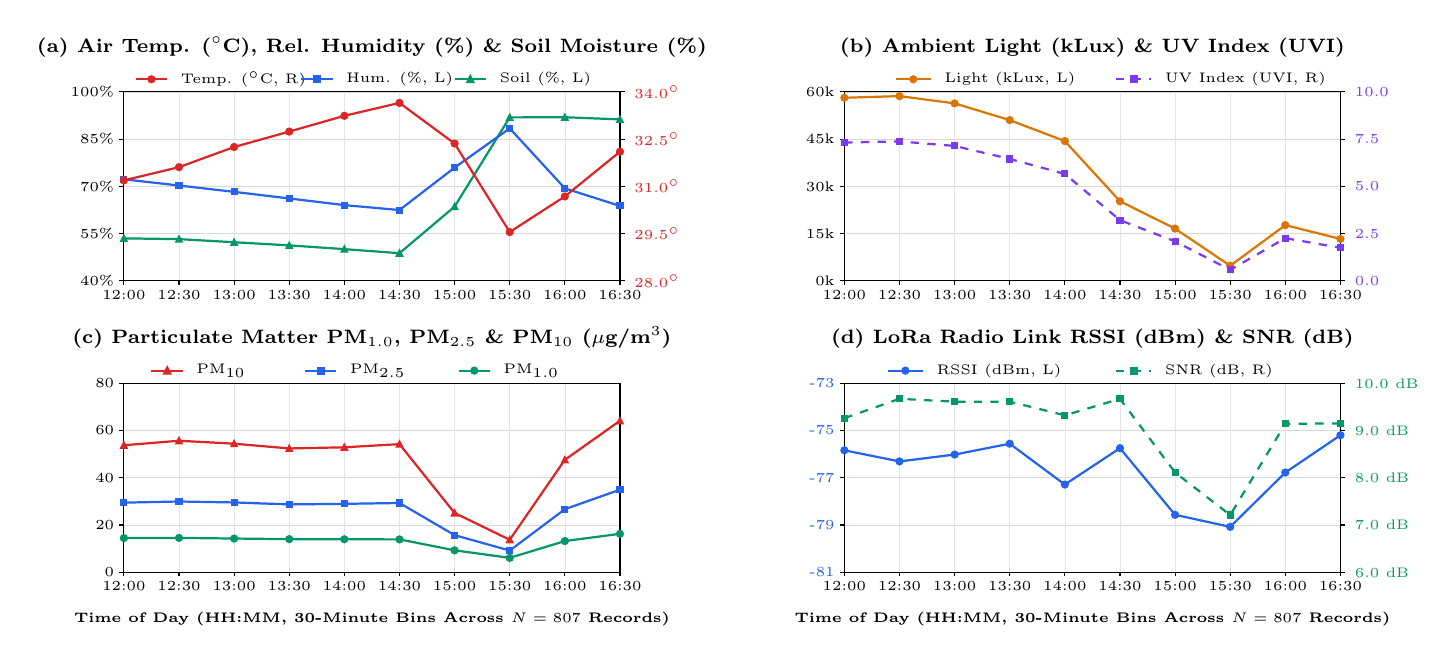
\begin{tikzpicture}[x=1cm,y=1cm,font=\scriptsize]
\definecolor{cRed}{RGB}{220,38,38}
\definecolor{cBlue}{RGB}{37,99,235}
\definecolor{cGreen}{RGB}{5,150,105}
\definecolor{cOrange}{RGB}{217,119,6}
\definecolor{cPurple}{RGB}{124,58,237}

% ==================== PANEL (a): Temp (Right 28..34 C) & Hum/Soil (Left 40..100 %) ====================
\begin{scope}[shift={(1.05,3.70)}]
    \node[above,font=\scriptsize\bfseries] at (3.15,2.72) {(a) Air Temp. ($^\circ$C), Rel. Humidity (\%) \& Soil Moisture (\%)};
    % Legend
    \draw[cRed,thick] (0.15,2.56) -- (0.55,2.56); \fill[cRed] (0.35,2.56) circle (1.5pt);
    \node[anchor=west,font=\tiny] at (0.60,2.56) {Temp. ($^\circ$C, R)};
    \draw[cBlue,thick] (2.25,2.56) -- (2.65,2.56); \fill[cBlue] (2.40,2.51) rectangle (2.50,2.61);
    \node[anchor=west,font=\tiny] at (2.70,2.56) {Hum. (\%, L)};
    \draw[cGreen,thick] (4.20,2.56) -- (4.60,2.56); \fill[cGreen] (4.40,2.63) -- (4.34,2.51) -- (4.46,2.51) -- cycle;
    \node[anchor=west,font=\tiny] at (4.65,2.56) {Soil (\%, L)};

    % Grid & Axes (6.30 cm wide x 2.40 cm high)
    \foreach \y in {0.60,1.20,1.80,2.40} \draw[gray!30,very thin] (0,\y) -- (6.30,\y);
    \foreach \x in {0.70,1.40,2.10,2.80,3.50,4.20,4.90,5.60,6.30} \draw[gray!20,very thin] (\x,0) -- (\x,2.40);
    \draw[thin] (0,0) rectangle (6.30,2.40);

    % Left Y ticks: 40, 55, 70, 85, 100 (%)
    \foreach \v/\y in {40/0.00, 55/0.60, 70/1.20, 85/1.80, 100/2.40}
        \draw (-0.06,\y) -- (0,\y) node[left,font=\tiny] {\v\%};
    % Right Y ticks: 28.0, 29.5, 31.0, 32.5, 34.0 (C)
    \foreach \v/\y in {28.0/0.00, 29.5/0.60, 31.0/1.20, 32.5/1.80, 34.0/2.40}
        \draw (6.30,\y) -- (6.36,\y) node[right,font=\tiny,cRed] {\v$^\circ$};

    % X ticks (30-min bins 12:00..16:30)
    \foreach \lbl/\x in {12:00/0.00, 12:30/0.70, 13:00/1.40, 13:30/2.10, 14:00/2.80, 14:30/3.50, 15:00/4.20, 15:30/4.90, 16:00/5.60, 16:30/6.30}
        \draw (\x,-0.05) -- (\x,0) node[below,font=\tiny] {\lbl};

    % Soil line: y = (S - 40) * 0.04
    \draw[cGreen,thick] (0.00,0.5396) -- (0.70,0.5300) -- (1.40,0.4904) -- (2.10,0.4508) -- (2.80,0.4028) -- (3.50,0.3512) -- (4.20,0.9432) -- (4.90,2.0760) -- (5.60,2.0780) -- (6.30,2.0504);
    \foreach \x/\y in {0.00/0.5396, 0.70/0.5300, 1.40/0.4904, 2.10/0.4508, 2.80/0.4028, 3.50/0.3512, 4.20/0.9432, 4.90/2.0760, 5.60/2.0780, 6.30/2.0504}
        \fill[cGreen,shift={(\x,\y)}] (0,0.06) -- (-0.055,-0.045) -- (0.055,-0.045) -- cycle;

    % Humidity line: y = (H - 40) * 0.04
    \draw[cBlue,thick] (0.00,1.2900) -- (0.70,1.2108) -- (1.40,1.1304) -- (2.10,1.0464) -- (2.80,0.9620) -- (3.50,0.8992) -- (4.20,1.4380) -- (4.90,1.9368) -- (5.60,1.1748) -- (6.30,0.9520);
    \foreach \x/\y in {0.00/1.2900, 0.70/1.2108, 1.40/1.1304, 2.10/1.0464, 2.80/0.9620, 3.50/0.8992, 4.20/1.4380, 4.90/1.9368, 5.60/1.1748, 6.30/0.9520}
        \fill[cBlue,shift={(\x,\y)}] (-0.045,-0.045) rectangle (0.045,0.045);

    % Temp line: y = (T - 28.0) * 0.40
    \draw[cRed,thick] (0.00,1.2760) -- (0.70,1.4440) -- (1.40,1.7000) -- (2.10,1.8960) -- (2.80,2.0960) -- (3.50,2.2600) -- (4.20,1.7440) -- (4.90,0.6200) -- (5.60,1.0720) -- (6.30,1.6400);
    \foreach \x/\y in {0.00/1.2760, 0.70/1.4440, 1.40/1.7000, 2.10/1.8960, 2.80/2.0960, 3.50/2.2600, 4.20/1.7440, 4.90/0.6200, 5.60/1.0720, 6.30/1.6400}
        \fill[cRed] (\x,\y) circle (1.5pt);
\end{scope}

% ==================== PANEL (b): Light (Left 0..60 kLux) & UV Index (Right 0..10 UVI) ====================
\begin{scope}[shift={(10.20,3.70)}]
    \node[above,font=\scriptsize\bfseries] at (3.15,2.72) {(b) Ambient Light (kLux) \& UV Index (UVI)};
    % Legend
    \draw[cOrange,thick] (0.65,2.56) -- (1.10,2.56); \fill[cOrange] (0.875,2.56) circle (1.5pt);
    \node[anchor=west,font=\tiny] at (1.15,2.56) {Light (kLux, L)};
    \draw[cPurple,thick,dashed] (3.45,2.56) -- (3.90,2.56); \fill[cPurple] (3.63,2.51) rectangle (3.73,2.61);
    \node[anchor=west,font=\tiny] at (3.95,2.56) {UV Index (UVI, R)};

    % Grid & Axes
    \foreach \y in {0.60,1.20,1.80,2.40} \draw[gray!30,very thin] (0,\y) -- (6.30,\y);
    \foreach \x in {0.70,1.40,2.10,2.80,3.50,4.20,4.90,5.60,6.30} \draw[gray!20,very thin] (\x,0) -- (\x,2.40);
    \draw[thin] (0,0) rectangle (6.30,2.40);

    % Left Y ticks: 0, 15, 30, 45, 60 (kLux)
    \foreach \v/\y in {0/0.00, 15/0.60, 30/1.20, 45/1.80, 60/2.40}
        \draw (-0.06,\y) -- (0,\y) node[left,font=\tiny] {\v k};
    % Right Y ticks: 0.0, 2.5, 5.0, 7.5, 10.0 (UVI)
    \foreach \v/\y in {0.0/0.00, 2.5/0.60, 5.0/1.20, 7.5/1.80, 10.0/2.40}
        \draw (6.30,\y) -- (6.36,\y) node[right,font=\tiny,cPurple] {\v};

    % X ticks
    \foreach \lbl/\x in {12:00/0.00, 12:30/0.70, 13:00/1.40, 13:30/2.10, 14:00/2.80, 14:30/3.50, 15:00/4.20, 15:30/4.90, 16:00/5.60, 16:30/6.30}
        \draw (\x,-0.05) -- (\x,0) node[below,font=\tiny] {\lbl};

    % Light line: y = L_kLux * 0.04
    \draw[cOrange,thick] (0.00,2.3252) -- (0.70,2.3464) -- (1.40,2.2540) -- (2.10,2.0416) -- (2.80,1.7752) -- (3.50,1.0112) -- (4.20,0.6636) -- (4.90,0.1920) -- (5.60,0.7080) -- (6.30,0.5324);
    \foreach \x/\y in {0.00/2.3252, 0.70/2.3464, 1.40/2.2540, 2.10/2.0416, 2.80/1.7752, 3.50/1.0112, 4.20/0.6636, 4.90/0.1920, 5.60/0.7080, 6.30/0.5324}
        \fill[cOrange] (\x,\y) circle (1.5pt);

    % UVI line: y = UVI * 0.24
    \draw[cPurple,thick,dashed] (0.00,1.7568) -- (0.70,1.7712) -- (1.40,1.7136) -- (2.10,1.5480) -- (2.80,1.3584) -- (3.50,0.7704) -- (4.20,0.5016) -- (4.90,0.1392) -- (5.60,0.5424) -- (6.30,0.4200);
    \foreach \x/\y in {0.00/1.7568, 0.70/1.7712, 1.40/1.7136, 2.10/1.5480, 2.80/1.3584, 3.50/0.7704, 4.20/0.5016, 4.90/0.1392, 5.60/0.5424, 6.30/0.4200}
        \fill[cPurple,shift={(\x,\y)}] (-0.045,-0.045) rectangle (0.045,0.045);
\end{scope}

% ==================== PANEL (c): Fine Dust PM1.0, PM2.5, PM10 (0..80 ug/m3) ====================
\begin{scope}[shift={(1.05,0.00)}]
    \node[above,font=\scriptsize\bfseries] at (3.15,2.72) {(c) Particulate Matter $\text{PM}_{1.0}$, $\text{PM}_{2.5}$ \& $\text{PM}_{10}$ ($\mu\text{g/m}^3$)};
    % Legend
    \draw[cRed,thick] (0.35,2.56) -- (0.75,2.56); \fill[cRed] (0.55,2.63) -- (0.49,2.51) -- (0.61,2.51) -- cycle;
    \node[anchor=west,font=\tiny] at (0.80,2.56) {PM$_{10}$};
    \draw[cBlue,thick] (2.30,2.56) -- (2.70,2.56); \fill[cBlue] (2.45,2.51) rectangle (2.55,2.61);
    \node[anchor=west,font=\tiny] at (2.75,2.56) {PM$_{2.5}$};
    \draw[cGreen,thick] (4.25,2.56) -- (4.65,2.56); \fill[cGreen] (4.45,2.56) circle (1.5pt);
    \node[anchor=west,font=\tiny] at (4.70,2.56) {PM$_{1.0}$};

    % Grid & Axes
    \foreach \y in {0.60,1.20,1.80,2.40} \draw[gray!30,very thin] (0,\y) -- (6.30,\y);
    \foreach \x in {0.70,1.40,2.10,2.80,3.50,4.20,4.90,5.60,6.30} \draw[gray!20,very thin] (\x,0) -- (\x,2.40);
    \draw[thin] (0,0) rectangle (6.30,2.40);

    % Left Y ticks: 0, 20, 40, 60, 80 (ug/m3)
    \foreach \v/\y in {0/0.00, 20/0.60, 40/1.20, 60/1.80, 80/2.40}
        \draw (-0.06,\y) -- (0,\y) node[left,font=\tiny] {\v};

    % X ticks
    \foreach \lbl/\x in {12:00/0.00, 12:30/0.70, 13:00/1.40, 13:30/2.10, 14:00/2.80, 14:30/3.50, 15:00/4.20, 15:30/4.90, 16:00/5.60, 16:30/6.30}
        \draw (\x,-0.05) -- (\x,0) node[below,font=\tiny] {\lbl};
    \node[below,font=\tiny\bfseries] at (3.15,-0.38) {Time of Day (HH:MM, 30-Minute Bins Across $N=807$ Records)};

    % PM10 line: y = PM10 * 0.03
    \draw[cRed,thick] (0.00,1.6122) -- (0.70,1.6695) -- (1.40,1.6320) -- (2.10,1.5717) -- (2.80,1.5861) -- (3.50,1.6263) -- (4.20,0.7524) -- (4.90,0.4119) -- (5.60,1.4271) -- (6.30,1.9230);
    \foreach \x/\y in {0.00/1.6122, 0.70/1.6695, 1.40/1.6320, 2.10/1.5717, 2.80/1.5861, 3.50/1.6263, 4.20/0.7524, 4.90/0.4119, 5.60/1.4271, 6.30/1.9230}
        \fill[cRed,shift={(\x,\y)}] (0,0.06) -- (-0.055,-0.045) -- (0.055,-0.045) -- cycle;

    % PM2.5 line: y = PM2.5 * 0.03
    \draw[cBlue,thick] (0.00,0.8835) -- (0.70,0.8979) -- (1.40,0.8859) -- (2.10,0.8610) -- (2.80,0.8682) -- (3.50,0.8790) -- (4.20,0.4707) -- (4.90,0.2751) -- (5.60,0.8001) -- (6.30,1.0479);
    \foreach \x/\y in {0.00/0.8835, 0.70/0.8979, 1.40/0.8859, 2.10/0.8610, 2.80/0.8682, 3.50/0.8790, 4.20/0.4707, 4.90/0.2751, 5.60/0.8001, 6.30/1.0479}
        \fill[cBlue,shift={(\x,\y)}] (-0.045,-0.045) rectangle (0.045,0.045);

    % PM1.0 line: y = PM1.0 * 0.03
    \draw[cGreen,thick] (0.00,0.4335) -- (0.70,0.4356) -- (1.40,0.4275) -- (2.10,0.4200) -- (2.80,0.4182) -- (3.50,0.4167) -- (4.20,0.2781) -- (4.90,0.1821) -- (5.60,0.3954) -- (6.30,0.4875);
    \foreach \x/\y in {0.00/0.4335, 0.70/0.4356, 1.40/0.4275, 2.10/0.4200, 2.80/0.4182, 3.50/0.4167, 4.20/0.2781, 4.90/0.1821, 5.60/0.3954, 6.30/0.4875}
        \fill[cGreen] (\x,\y) circle (1.5pt);
\end{scope}

% ==================== PANEL (d): LoRa Link RSSI (Left -81..-73 dBm) & SNR (Right 6..10 dB) ====================
\begin{scope}[shift={(10.20,0.00)}]
    \node[above,font=\scriptsize\bfseries] at (3.15,2.72) {(d) LoRa Radio Link RSSI (dBm) \& SNR (dB)};
    % Legend
    \draw[cBlue,thick] (0.55,2.56) -- (1.00,2.56); \fill[cBlue] (0.775,2.56) circle (1.5pt);
    \node[anchor=west,font=\tiny] at (1.05,2.56) {RSSI (dBm, L)};
    \draw[cGreen,thick,dashed] (3.45,2.56) -- (3.90,2.56); \fill[cGreen] (3.63,2.51) rectangle (3.73,2.61);
    \node[anchor=west,font=\tiny] at (3.95,2.56) {SNR (dB, R)};

    % Grid & Axes
    \foreach \y in {0.60,1.20,1.80,2.40} \draw[gray!30,very thin] (0,\y) -- (6.30,\y);
    \foreach \x in {0.70,1.40,2.10,2.80,3.50,4.20,4.90,5.60,6.30} \draw[gray!20,very thin] (\x,0) -- (\x,2.40);
    \draw[thin] (0,0) rectangle (6.30,2.40);

    % Left Y ticks: -81, -79, -77, -75, -73 (dBm)
    \foreach \v/\y in {-81/0.00, -79/0.60, -77/1.20, -75/1.80, -73/2.40}
        \draw (-0.06,\y) -- (0,\y) node[left,font=\tiny,cBlue] {\v};
    % Right Y ticks: 6.0, 7.0, 8.0, 9.0, 10.0 (dB)
    \foreach \v/\y in {6.0/0.00, 7.0/0.60, 8.0/1.20, 9.0/1.80, 10.0/2.40}
        \draw (6.30,\y) -- (6.36,\y) node[right,font=\tiny,cGreen] {\v\text{ dB}};

    % X ticks
    \foreach \lbl/\x in {12:00/0.00, 12:30/0.70, 13:00/1.40, 13:30/2.10, 14:00/2.80, 14:30/3.50, 15:00/4.20, 15:30/4.90, 16:00/5.60, 16:30/6.30}
        \draw (\x,-0.05) -- (\x,0) node[below,font=\tiny] {\lbl};
    \node[below,font=\tiny\bfseries] at (3.15,-0.38) {Time of Day (HH:MM, 30-Minute Bins Across $N=807$ Records)};

    % RSSI line: y = (RSSI + 81) * 0.30
    \draw[cBlue,thick] (0.00,1.5480) -- (0.70,1.4070) -- (1.40,1.4940) -- (2.10,1.6320) -- (2.80,1.1130) -- (3.50,1.5750) -- (4.20,0.7290) -- (4.90,0.5760) -- (5.60,1.2660) -- (6.30,1.7400);
    \foreach \x/\y in {0.00/1.5480, 0.70/1.4070, 1.40/1.4940, 2.10/1.6320, 2.80/1.1130, 3.50/1.5750, 4.20/0.7290, 4.90/0.5760, 5.60/1.2660, 6.30/1.7400}
        \fill[cBlue] (\x,\y) circle (1.5pt);

    % SNR line: y = (SNR - 6.0) * 0.60
    \draw[cGreen,thick,dashed] (0.00,1.9560) -- (0.70,2.2020) -- (1.40,2.1660) -- (2.10,2.1660) -- (2.80,1.9920) -- (3.50,2.2020) -- (4.20,1.2660) -- (4.90,0.7260) -- (5.60,1.8840) -- (6.30,1.8900);
    \foreach \x/\y in {0.00/1.9560, 0.70/2.2020, 1.40/2.1660, 2.10/2.1660, 2.80/1.9920, 3.50/2.2020, 4.20/1.2660, 4.90/0.7260, 5.60/1.8840, 6.30/1.8900}
        \fill[cGreen,shift={(\x,\y)}] (-0.045,-0.045) rectangle (0.045,0.045);
\end{scope}
\end{tikzpicture}
\caption{Half-hour time-of-day line charts (\texttt{12:00} to \texttt{16:30}) of the three-day field test dataset (\texttt{gateway\_weather\_log.csv}, Node 1, $N = 807$ records across 10 thirty-minute bins: $n = 31, 89, 89, 87, 90, 89, 93, 90, 90, 59$) showing (a) Air Temperature ($^\circ$C, right axis) vs. Relative Humidity and Soil Moisture (\%, left axis), (b) Ambient Light (kLux, left axis) and UV Index (UVI, right axis), (c) Fine Dust $\text{PM}_{1.0}$, $\text{PM}_{2.5}$, and $\text{PM}_{10}$ ($\mu\text{g/m}^3$), and (d) LoRa RSSI (dBm, left axis) and SNR (dB, right axis).}
\label{fig:dataset_chart}
\end{figure}

\subsection{Local Climate, Soil, Dust, and Radio Link Observations}
As shown in Table~\ref{tab:dataset} and the line charts in Fig.~\ref{fig:dataset_chart}, the sensor node recorded clear daily weather patterns across all three afternoons:
\begin{enumerate}
    \item \textbf{Air Temperature and Relative Humidity (AM2301B, Fig.~\ref{fig:dataset_chart}(a)):} Daily temperature ranges were $28.84\text{--}34.24\,^\circ\text{C}$ on Day 1, $28.81\text{--}34.21\,^\circ\text{C}$ on Day 2, and $28.50\text{--}34.08\,^\circ\text{C}$ on Day 3, while relative humidity ranged from $59.92\text{--}95.57\%$, $61.17\text{--}95.66\%$, and $60.85\text{--}94.59\%$. Temperature and relative humidity moved in opposite directions: as afternoon temperature rose from $30.87\text{--}31.66\,^\circ\text{C}$ at midday to a peak of $34.08\text{--}34.24\,^\circ\text{C}$ around \texttt{14:15--14:55} (bin mean $33.65\,^\circ\text{C}$ at \texttt{14:30}), relative humidity dropped to $59.92\text{--}60.85\%$ (bin mean $62.48\%$). Later, between \texttt{15:25} and \texttt{15:50}, temperature cooled to $28.50\text{--}28.84\,^\circ\text{C}$ (bin mean $29.55\,^\circ\text{C}$ at \texttt{15:30}) while relative humidity rose to $94.59\text{--}95.66\%$ (bin mean $88.42\%$).
    \item \textbf{Ambient Light (BH1750) and UV Index (LTR390, Fig.~\ref{fig:dataset_chart}(b)):} Light intensity and UV index closely followed the same daily curve. Daily light ranges were $2096.00\text{--}63,195.30\text{ Lux}$ (UVI $0.00\text{--}8.18$) on Day 1, $2084.70\text{--}63,462.30\text{ Lux}$ (UVI $0.00\text{--}8.05$) on Day 2, and $2047.90\text{--}64,645.80\text{ Lux}$ (UVI $0.00\text{--}8.46$) on Day 3. Both readings reached their highest levels around \texttt{12:07--12:30} (bin mean $58.66\text{ kLux}$ and UVI $7.38$ at \texttt{12:30}), dropped sharply during the cloudy/wet period at \texttt{15:30} (bin mean $4.80\text{ kLux}$ and UVI $0.58$, reaching UVI $0.00$ in 8 packets), and rose slightly to $17.70\text{ kLux}$ (UVI $2.26$) at \texttt{16:00} before sunset.
    \item \textbf{Soil Moisture (Grove Sensor) and Fine Dust (APM10, Fig.~\ref{fig:dataset_chart}(a, c)):} Soil moisture began around $52.9\text{--}53.2\%$ at midday, slowly dried to $47.20\text{--}48.00\%$ by \texttt{14:55--15:00} (bin mean $48.78\%$ at \texttt{14:30}), and then jumped to $90.4\text{--}92.2\%$ at \texttt{15:10--15:30} after watering/rain, staying at $90.1\text{--}92.8\%$ for the rest of the afternoon (bin means $91.90\text{--}91.95\%$ at \texttt{15:30--16:00}). At the same time, $\text{PM}_{1.0}$ ($3.00\text{--}21.00\,\mu\text{g/m}^3$), $\text{PM}_{2.5}$ ($5.00\text{--}49.00\,\mu\text{g/m}^3$), and $\text{PM}_{10}$ ($8.00\text{--}112.00\,\mu\text{g/m}^3$) moved together, dropping to their lowest levels ($3$, $5$, and $8\,\mu\text{g/m}^3$; bin means $6.07$, $9.17$, and $13.73\,\mu\text{g/m}^3$ at \texttt{15:30}) during the high-humidity period around \texttt{15:30--15:45}.
    \item \textbf{LoRa Radio Link Performance (RSSI and SNR, Fig.~\ref{fig:dataset_chart}(d)):} Across all 807 packets, \texttt{RSSI} stayed between $-90.00$ and $-65.00\text{ dBm}$ (mean $-76.77\text{ dBm}$, median $-77.00\text{ dBm}$ each day, $\text{SD} = 4.00\text{ dBm}$) and \texttt{SNR} remained positive between $2.80$ and $13.50\text{ dB}$ (mean $9.05\text{ dB}$). Compared with the $-114$ to $-124\text{ dB}$ RSSI levels where Hidayat et al. \cite{hidayat2019} saw 20\%--80\% packet loss, our LoRa link maintained a strong signal and stable 1-minute data delivery.
\end{enumerate}

\section{Discussion and Limitations}

\subsection{Addressing Literature Gaps and Design Benefits}
The proposed system addresses all three gaps identified in Section II. First, unlike outdoor weather stations focused mainly on wind and rain \cite{dajnowski2024, zennaro2025, lopez2025, pietrosemoli2019, murdyantoro2019} without UV index or deployed fine dust sensors, our node combines five sensors measuring eight environmental parameters (air temperature, relative humidity, ambient light, UV index, soil moisture, $\text{PM}_{1.0}$, $\text{PM}_{2.5}$, and $\text{PM}_{10}$) suitable for both greenhouses and open farms. Second, the ESP32-S3-N16R8 overcomes the Arduino memory limits reported in \cite{dajnowski2024} and supports a compact 26-byte binary protocol, dual gateway storage (MicroSD card plus 16 MB internal flash backup and a 50-record RAM buffer), and automatic switching between ThingSpeak Cloud and a local offline web dashboard. Third, combining direct electrical power with a 10,000 mAh Li-Po backup battery, RTC-saved packet counters, and 60-second deep sleep keeps the sensor node running smoothly during power outages.

\subsection{Limitations}
First, our current prototype does not include wind speed and wind direction sensors, unlike \cite{dajnowski2024, zennaro2025, lopez2025, pietrosemoli2019, murdyantoro2019}. While wind is minimal inside closed greenhouses, it is an important factor for open-field farms because wind affects plant water loss and the metabolism rate of many plant species \cite{dajnowski2024}. Second, although the LoRa module and 525 MHz 3.5 dBi antenna can theoretically reach \textbf{5--10 km} in open rural areas---similar to the 5--10 km rural links demonstrated in \cite{lopez2025} and ranges quoted in \cite{dajnowski2024, murdyantoro2019}---our field tests were conducted in an \textbf{urban environment}, where dense buildings and obstacles currently limit the effective transmission distance to about \textbf{1 km}, consistent with the urban signal loss reported by Hidayat et al. \cite{hidayat2019}.

\section{Conclusion}
This paper presented a low-power LoRa-based climate monitoring system for large-scale farms and greenhouses where Wi-Fi and cellular coverage is limited. Built on the ESP32-S3-N16R8 microcontroller and MKE-M24 Ra-02SH (Semtech SX1278) LoRa module, the system connects AM2301B, BH1750, LTR390, Grove Soil Moisture, and APM10 sensors with DS1307 RTC timekeeping, a 10,000 mAh Li-Po backup battery, deep-sleep power management, dual MicroSD/flash gateway storage, ThingSpeak cloud streaming, and a local backup web dashboard. Across a three-day urban field test (November 5--7, 2026), the station reliably logged 807 packets at a 60.10 s mean interval with a mean RSSI of $-76.77$ dBm and mean SNR of 9.05 dB. Future work will add wind sensors for open farms, test multi-hop repeater forwarding, and evaluate 5--10 km range in open rural farmland.

\bibliographystyle{IEEEtran}
\bibliography{Paper_ref}

\clearpage
\begin{center}
{\large\textbf{AI USAGE DECLARATION \enspace|\enspace IOT102 \enspace|\enspace Fall 2026}}
\end{center}
\noindent\rule{\textwidth}{0.6pt}

\vspace{8pt}
\noindent\textbf{Group: 2}

\vspace{8pt}
\noindent\textbf{Topic: LoRa-Based Climate Monitoring System for Large-Scale Farms and Greenhouses}

\vspace{10pt}
\noindent\uncheckedbox\enspace We did NOT use AI-generated tools in this report.

\vspace{6pt}
\noindent\uncheckedbox\enspace We DO use AI (check all appropriate purposes)

\vspace{6pt}
\noindent\hspace*{1.5em}Tools: [ChatGPT / Claude / Copilot / Gemini /...]

\vspace{6pt}
\noindent\hspace*{1.5em}Purpose:

\vspace{4pt}
\noindent\hspace*{2.5em}\uncheckedbox\enspace System / architecture design exploration

\vspace{4pt}
\noindent\hspace*{2.5em}\uncheckedbox\enspace Hardware / protocol selection research

\vspace{4pt}
\noindent\hspace*{2.5em}\uncheckedbox\enspace Code generation / debugging

\vspace{4pt}
\noindent\hspace*{2.5em}\uncheckedbox\enspace Data analysis support

\vspace{4pt}
\noindent\hspace*{2.5em}\uncheckedbox\enspace Literature exploration

\vspace{4pt}
\noindent\hspace*{2.5em}\uncheckedbox\enspace Technical writing / language editing

\vspace{4pt}
\noindent\hspace*{2.5em}\uncheckedbox\enspace Other: .................................................

\vspace{10pt}
\noindent We confirm that all engineering decisions, evaluation results, and conclusions presented in this report are the product of the team's own thinking..

\vspace{6pt}
\noindent\rule{\textwidth}{0.6pt}

\end{document}
